94. $\cfrac{5}{2x+1}+\cfrac{2}{7x-1}\leqslant3\Leftrightarrow\cfrac{35x-5+4x+2-42x^2+6x-21x+3}{(2x+1)(7x-1)}\leqslant 0\Leftrightarrow
\cfrac{6x(4-7x)}{(2x+1)(7x-1)}\leqslant 0.$ Применив метод интервалов, найдём ответ:
\begin{figure}[ht!]
\center{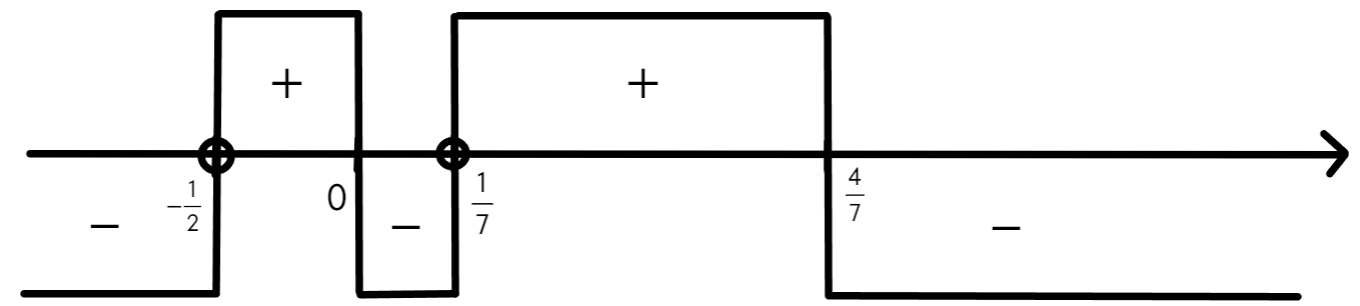
\includegraphics[scale=0.35]{int94.png}}
\end{figure}
$x\in\left(-\infty;-\cfrac{1}{2}
ight)\cup\left[0;\cfrac{1}{7}
ight)\cup\left(\cfrac{4}{7};+\infty
ight).$\\
